\documentclass[12pt,oneside]{article}
\usepackage{light}
\newcommand{\mfigure}[3]{\bigskip\centerline{\resizebox{#1}{#2}{\includegraphics{#3}}}\bigskip}
\newcommand{\hint}[1]{({\it Hint: #1})}
\newcommand{\brule}[1]{\underline{\hspace{#1}}}
\newcommand{\ang}[1]{\left< #1 \right>}
\newcommand{\beats}{\rightarrow}

\newenvironment{falseproof}
{\begin{proof}[False proof]}
{\end{proof}}

\showsolutions
%\hidesolutions

\begin{document}
\generic{Midterm Practice Problems}{October 21, 2010}

\instatements{
\vspace{24pt}
\textbf{Name:} \rule{5in}{0.5pt}

\begin{itemize}

\item This quiz is \textbf{closed book}, but you may have one $8.5
\times 11$'' sheet with notes in your own handwriting on both sides.

\item Calculators are not allowed.

\item You may assume all of the results presented in class.

\item Please show your work.  Partial credit cannot be given for a wrong
answer if your work isn't shown.

\item Write your solutions in the space provided.  If you
need more space, write on the back of the sheet containing the
problem.  Please keep your entire answer to a problem on that
problem's page.

\item Be neat and write legibly.  You will be graded not only on the
correctness of your answers, but also on the clarity with which you
express them.

\item If you get stuck on a problem, move on to others. The problems 
are not arranged in order of difficulty.

\end{itemize}

\vspace{0.25in}

%\begin{center}
%{\large
%\begin{tabular}{|c|c|c|c|}
%\hline
%Problem & Points & Grade & Grader \\ \hline \hline
%1 & 10 & & \\ \hline
%2 & 15 & & \\ \hline
%3 & 20 & & \\ \hline
%4 & 10 & & \\ \hline
%5 & 15 & & \\ \hline
%6 & 10 & & \\ \hline
%7 & 20 & & \\ \hline
%Total & 100 & & \\ \hline
%\end{tabular}
%}
%\end{center}
}
\instatements{\newpage}


%%%%%%%%%%%%%%%%%%%%%%%%%%%%%%%%%%%%%%%%%%%%%%%%%%%%%%%%%%%%%%%%%%%%%
% taken from: new problem
% comments: boolean logic
%
\instatements{\newpage}
\begin{problem}{10}
In problem set 1 you showed that the $\nand$ operator by itself can be used to write equivalent expressions for all other Boolean logical operators. We call such an operator \emph{universal}. Another universal operator is $\nor$, defined such that $P \nor Q \iff \neg (P \lor Q)$.

Show how to express $P \land Q$ in terms of: $\nor$, $P$, $Q$, and grouping parentheses.

\solution[\vspace{3in}]{$(\neg P) \nor (\neg Q) = (P \nor P) \nor (Q \nor Q)$.}

\end{problem}


%%%%%%%%%%%%%%%%%%%%%%%%%%%%%%%%%%%%%%%%%%%%%%%%%%%%%%%%%%%%%%%%%%%%%
% taken from: new problem
% comments: strong induction and number theory
%
\begin{problem}{15}
We define the sequence of numbers
\begin{eqnarray*}
a_n = \begin{cases}
  1                                    &  \text{if $0 \leq n \leq 3$,}\\
  a_{n-1} + a_{n-2} + a_{n-3}+ a_{n-4} &  \text{if $n \geq 4$.}
 \end{cases}
\end{eqnarray*}

Prove that $a_n \equiv 1 \pmod{3}$ for all $n\geq 0$. 

\solution[\newpage]{
Proof by strong induction. Let $P(n)$ be the 
predicate that $a_n \equiv 1 \pmod{3}$.

Base case: For $0\leq n\leq 3$, $a_n=1$ and is therefore 
$\equiv 1 \pmod{3}$.

Inductive step: For $n \geq 4$, assume $P(k)$ for $0\leq k\leq n$ 
in order to prove $P(n+1)$.

In particular, since each of $a_{n-4}$, $a_{n-3}$, $a_{n-2}$ and $a_{n-1}$ 
is $\equiv 1 \pmod{3}$, their sum must be $\equiv 4 \equiv 1 \pmod{3}$.
Therefore, $a_n \equiv 1 \pmod{3}$ and $P(n+1)$ holds.}

\end{problem}


%%%%%%%%%%%%%%%%%%%%%%%%%%%%%%%%%%%%%%%%%%%%%%%%%%%%%%%%%%%%%%%%%%%%%
% taken from: new problem
% comments: 
%
\begin{problem}{20}\label{slipped_disc}
The Slipped Disc Puzzle\texttrademark\ consists of a track holding 9 
circular tiles. In the middle is a disc that can slide left and right and rotate 
$180\,^{\circ}$
to change the positions of \emph{exactly} four tiles. As shown below, there are 
three ways to manipulate the puzzle:

\begin{description}
\item[Shift Right:] The center disc is moved one unit to the right (if there is space)
\item[Rotate Disc:] The four tiles in the center disc are reversed
\item[Shift Left:] The center disc is moved one unit to the left (if there is space)
\end{description} 

\begin{center}
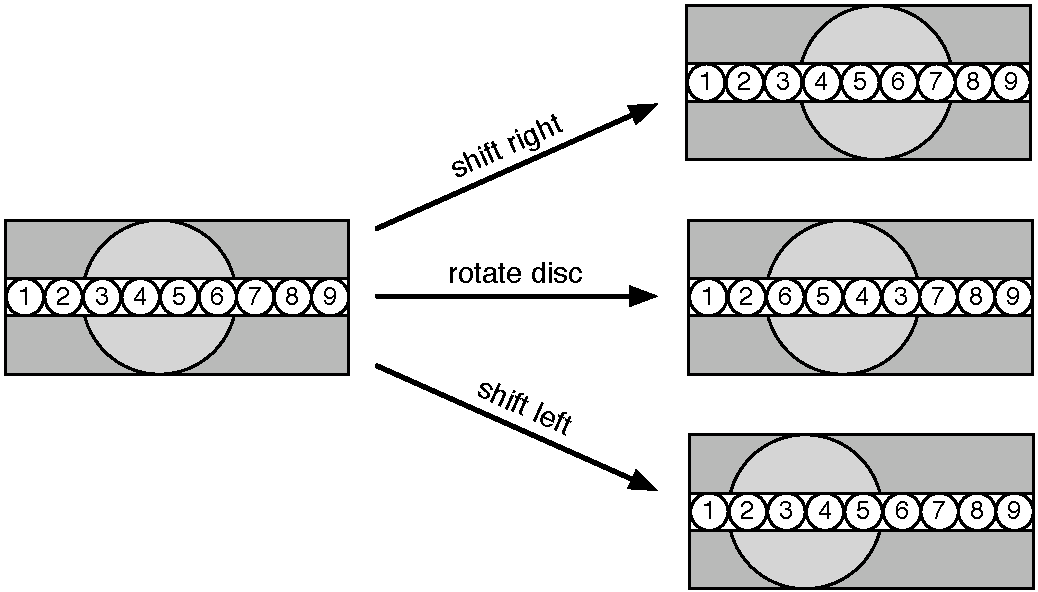
\includegraphics[width=5in]{1d-puzzle-transitions}
\end{center}

Prove that if the puzzle starts in an initial state with all but tiles 1 
and 2 in their natural order, then it is impossible to reach a goal state 
where all the tiles are in their natural order.  The initial and goal states are shown below:

\begin{center}
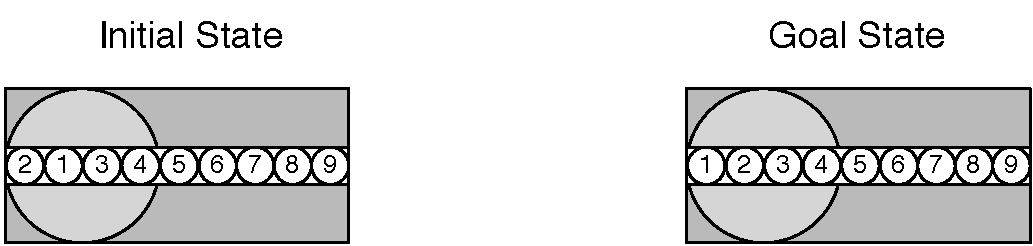
\includegraphics[width=5in]{1d-puzzle-challenge}
\end{center}

Write your proof on the next page...

\solution[\newpage]{
Order the tiles from left to right in the puzzle. Define an \emph{inversion} to be a pair of tiles that is out of their natural order (e.g. 4 appearing to the left of 3). 
\begin{lemma*}
Starting from the initial state there is an odd number of inversions after any number of transitions.
\end{lemma*}
\begin{proof}
The proof is by induction.  Let $P(n)$ be the proposition that starting from the initial state there is an odd number of inversions after $n$ transitions.

{\bf Base case:} After 0 transitions, there is one inversion, so $P(0)$ 
holds.

{\bf Inductive step:} Assume $P(n)$ is true.  Say we have a configuration 
that is reachable after $n + 1$ transitions.
\begin{enumerate}
\item Case 1: The last transition was a shift left or shift right

In this case, the left-to-right order of the discs does not change and thus the number of inversions remains the same as in 

\item The last transition was a rotate disc.

In this case, six pairs of disks switch order.  If there were $x$ inversions among these pairs after $n$ transitions, there will be $6 - x$ inversions after the reversal. If $x$ is odd, $6-x$ is odd, so after $n+1$ transitions the number of inversions is odd.
\end{enumerate}
\end{proof}

Conclusion: Since all reachable states have an odd number of inversions and the goal state has an even number of inversions (specifically 0), the goal state cannot be reached.
}

\instatements{
\newpage
{\bf room for problem \ref{slipped_disc}...}
}

\end{problem}



%%%%%%%%%%%%%%%%%%%%%%%%%%%%%%%%%%%%%%%%%%%%%%%%%%%%%%%%%%%%%%%%%%%%%
% taken from: new problem
% comments: number theory
%
\newpage
\begin{problem}{10} 
Find the multiplicative inverse of 17 modulo 72 in the range 
$\{0,1,\ldots,71\}$.

\solution[\newpage]{Since 17 and $72=2^3 3^2$ are relatively prime,
an inverse exists and can be found by either Euler's theorem or the
Pulverizer.

{\bf Solution 1: Euler's Theorem}

\begin{align*}
\phi(72) & = \phi(2^3 \cdot 3^2) &\\
          & = \phi(2^3) \cdot \phi(3^2) 
                  & \text{(since $2^3$ and $3^2$ are rel. prime)}\\
          & = (2^3 - 2^2)(3^2 - 3^1)
                  & \text{(since $2$ and $3$ are prime)}\\
          & = 4 \cdot 6 = 24 &
\end{align*}

Therefore, $17^{\phi(72)-1}=17^{23}$ is {\it an} inverse of 17.  To find
{\it the} inverse in the range $\{0,1,\ldots,71\}$ we take the remainder
using the method of repeated squaring:

\begin{align*}
17   & =       17 &\\
17^2 & =       289 &\\
     & \equiv  1 & \text{(since $289=4 \cdot 72 + 1$)}\\
17^4 & \equiv 1^2 = 1 &\\
17^8 & \equiv 1 &\\
& \ldots etc.&
\end{align*}

Therefore the inverse of 17 in the range $\{0,1,\ldots,71\}$ is given by,
\begin{align*}
17^{23} & = 17^{16} 17^{4} 17^{2} 17^{1} \\ 
        & \equiv 1 \cdot 1 \cdot 1 \cdot 17 \\
        & = 17
\end{align*}

{\bf Solution 2: The Pulverizer}
\[
\begin{array}{ccccrcl}
x & \quad & y & \quad & \rem{x}{y} & = & x - q \cdot y \\ \hline
72 && 17 && 4   & = &   72 - 4 \cdot 17 \\
17 && 4  && 1   & = &   17 - 4 \cdot 4 \\
&&&&            & = &   17 - 4 \cdot (72 - 4 \cdot 17) \\
&&&&            & = &   17 \cdot 17 - 4 \cdot 72 \\
4 && 1 && 0
\end{array}
\]

Since $17^2 - 4 \cdot 72 = 1$, $17^2 \equiv 1 \pmod{72}$ and so 17
is self inverse.
}

\end{problem}

%%%%%%%%%%%%%%%%%%%%%%%%%%%%%%%%%%%%%%%%%%%%%%%%%%%%%%%%%%%%%%%%%%%%%
% taken from: new problem
% comments: elementary graph theory
%
\begin{problem}{15}
Consider a graph representing the main campus buildings at MIT.

\vspace{18pt}
\centerline{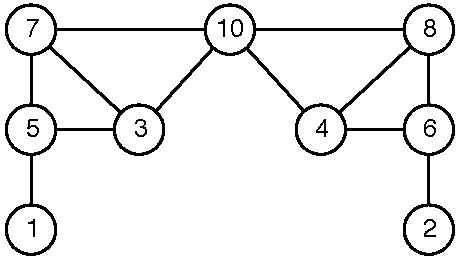
\includegraphics[width=3in]{maclaurin-graph}}
\vspace{18pt}

\bparts

\ppart{3} Is this graph bipartite? Provide a brief argument for your answer.
\solution[\vspace{1.5in}]{No, there is an odd-length cycle}

\ppart{4} Does this graph have an Euler circuit? Provide a brief argument for your answer.
\solution[\vspace{1.5in}]{This graph does not have an Euler circuit because there are vertices with odd degree}

\newpage
\textbf{Problem 5 continued...}

Now suppose each building has separate mail collection and drop-off boxes and each collection box has a single package destined for a unique drop-off box (i.e. a permutation). We can model this as a permutation routing problem by treating the buildings as switches, attaching an input and output terminal to each of the nine buildings, and treating the existing edges as bidirectional as in the graph below:

\vspace{18pt}
\centerline{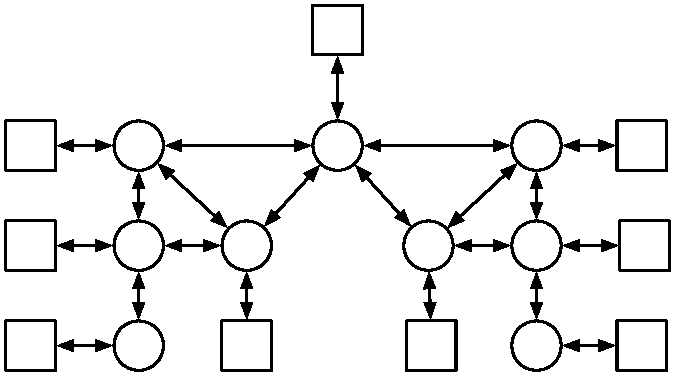
\includegraphics[width=4in]{maclaurin-routing}}
\vspace{18pt}

\ppart{4} Give the diameter of this graph:
\solution[\vspace{1in}]{The diameter is 8, the length of a shortest path between the terminals for buildings 1 and 2.}

\ppart{4} What is the max congestion of this graph? That is, in the worst case permutation, how many packages would need to pass through a single building?
Provide a brief argument for your answer.
\solution[\vspace{1in}]{The maximum congestion is 9. Consider a permutation where all the packages on the left side are destined for drop-offs on the right side and vice versa with the building 10 package destined for building 10.  In this case, all 9 packages must pass through building 10, giving a congestion of 9, which is the maximum for a graph with nine input-output pairs.
}

\eparts
\end{problem}
\newpage

%%%%%%%%%%%%%%%%%%%%%%%%%%%%%%%%%%%%%%%%%%%%%%%%%%%%%%%%%%%%%%%%%%%%%
% taken from: new problem
% comments: tournaments and relations
%
\begin{problem}{10}

A tournament graph $G=(V,E)$ is a directed graph such 
that there is either an edge from $u$ to $v$ or an edge from 
$v$ to $u$ for \textit{every} distinct pair of nodes $u$ 
and $v$. (The nodes represent players and an edge $u \beats v$ 
indicates that player $u$ beats player $v$.)

%Prove the proposition that if there exists a cycle 
%in a tournament graph $G$, then there exists a cycle of three 
%nodes in $G$. 
%\hint{Prove by contradiction by assuming there is a cycle
%but not a cycle of length 3 in $G$.}
%
%\solution[\newpage]{Assume for the purposes of obtaining a 
%contradiction that there was a directed cycle but no cycle of 
%length 3.  By the WOP there exists a minimum length cycle
%$v_1 \beats v_2 \ldots \beats v_h \beats v_1$ where $h>3$.
%
%Since $G$ is a tournament, either $v_1 \beats v_3$ or
%$v_3 \beats v_1$.  If $v_3 \beats v_1$ then a contradiction
%is obtained since $v_1 \beats v_2 \beats v_3 \beats v_1$ is
%a length 3 cycle.  Otherwise, a contradiction is obtained
%since $v_1 beats v_3 \beats \ldots \beats v_h \beats v_1$ 
%is a smaller cycle.}

Consider the ``beats'' relation implied by a tournament graph.  Indicate whether or not each of the following relational properties hold \emph{for all} tournament graphs and briefly explain your reasoning. You may assume that a player never plays herself.

\begin{enumerate}
\item {\bf transitive}
\solution[\vspace{1.75in}]{
The ``beats'' relation is not transitive because there could
exist a cycle of length 3 where $x$ beats $y$, $y$ beats $z$ and 
$z$ beats $x$.  By the definition of a tournament, $x$ cannot 
then beat $y$ in such a situation.}

\item {\bf symmetric}
\solution[\vspace{1.75in}]{
The ``beats'' relation is not symmetric by the definition of 
a tournament: if $x$ beats $y$ then $y$ does not beat $x$.}

\item {\bf antisymmetric}
\solution[\vspace{1.75in}]{
The ``beats'' relation is antisymmetric since for any distinct 
players $x$ and $y$, if $x$ beats $y$ then $y$ does not beat $x$.}

\item {\bf reflexive}
\solution[\vspace{1.75in}]{
The ``beats'' relation is not reflexive since a tournament
graph has no self-loops.}

\end{enumerate}
\end{problem}


%%%%%%%%%%%%%%%%%%%%%%%%%%%%%%%%%%%%%%%%%%%%%%%%%%%%%%%%%%%%%%%%%%%%%
% taken from: new problem
% comments: graph induction, outerplanar graphs
%
\instatements{\newpage}
\begin{problem}{20} An outerplanar graph is an undirected graph for 
which the vertices \emph{can be} placed on a circle in such a way 
that no edges (drawn as straight lines) cross each other.  For example, 
the complete graph on 4 vertices, $K_4$, is not outerplanar but any 
proper subgraph of $K_4$ with strictly fewer edges is outerplanar. Some
examples are provided below:

\vspace{18pt}
\centerline{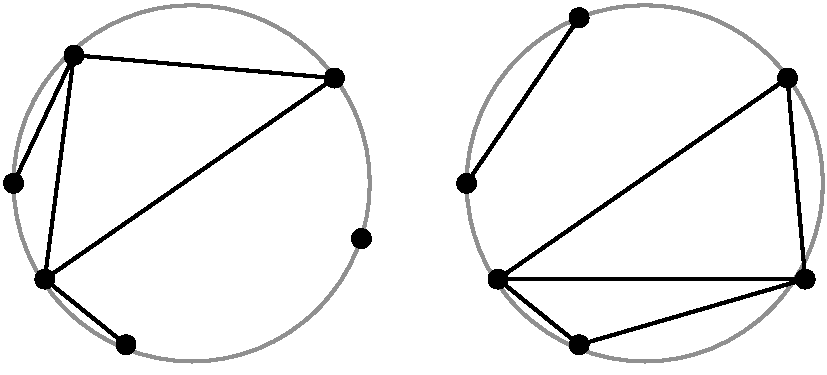
\includegraphics[width=3in]{outerplanar-graphs}}
\vspace{18pt}

Prove that any outerplanar graph is 3-colorable.  A fact you may use 
without proof is that any outerplanar graph has a vertex of degree at 
most 2.

\solution[\newpage]{
\begin{proof}
Proof by induction on the number of nodes $n$ with the induction 
hypothesis $P(n) =$ "every outerplanar graph with $n$ vertices is
3-colorable."

Base case: For $n=1$ the single node graph with no edges is 
trivially outerplanar and 3-colorable.

Inductive step: Assume $P(n)$ holds and let $G_{n+1}$ be an
outerplanar graph with $n+1$ vertices.  There must exist a vertex 
$v$ in $G_{n+1}$ with degree at most 2.  Removing $v$ and all its
incident edges leaves a subgraph $G_n$ with $n$ vertices.

Since $G_{n+1}$ could be drawn with its vertices on a circle and
its edges drawn as straight lines without intersections,
any subgraph can also be drawn in such a way and so $G_n$ is also
an outerplanar graph.  $P(n)$ implies $G_n$ is 3-colorable.  
Therefore we can color all the vertices in $G_{n+1}$ other than $v$
using only 3 colors and since $\deg(v) \leq 2$ we may color it a 
color different than the vertices adjacent to it using only 3 
colors.  Therefore, $G_{n+1}$ is 3-colorable and $P(n+1)$ holds.

\end{proof}
}


\end{problem}

\begin{problem}{10}
Give upper and lower bounds for the following expression which differ by at most 1.

% \hspace{0.5in} (\textit{Hint: $\frac{1}{(n+1)^2} \leq \frac{1}{n^2}$ for $n \geq 1$})

\[
\sum_{i=1}^{n} \frac{1}{i^3}
\]

\solution{
To find upper and lower bounds, we use the integral method:
\begin{align*}
\sum_{i=1}^{n} \frac{1}{i^3} & \leq 1+ \int_{1}^{n} \frac{1}{x^3} dx \\
& = 1 - \frac{1}{2}x^{-2} \Big |_{1}^{n} \\
& = 1 - \frac{1}{2}\left(\frac{1}{n^2} - 1\right) = \frac{3}{2} - \frac{1}{2n^2} \\
\sum_{i=1}^{n} \frac{1}{i^3} & \geq \frac{1}{n^3}+ \int_{1}^{n} \frac{1}{x^3} dx \\
& = \frac{1}{n^3}- \frac{1}{2}x^{-2}  \Big |_{1}^{n} \\
& = \frac{1}{n^3}- \frac{1}{2}\left(\frac{1}{n^2}-1\right) =  \frac{1}{2} + \frac{1}{n^3} - \frac{1}{2n^2}
\end{align*}
%
%Taking the difference between the upper and lower bounds we get:
%\[
%\left(\frac{3}{2} - \frac{1}{2n^2}\right) - \left(\frac{1}{2} + \frac{1}{n^3} - \frac{1}{2n^2}\right)
% = 1 - \left(\frac{1}{2n^2}+\frac{1}{n^3}\right)
%\]
%which is less than 1 for all n $\geq$ 1.
%
%We know that our bounds are within 1 of each other because:
%\begin{align*}
%upper - lower & = \left(\frac{n(n+1)}{2} + \frac{3}{2} - \frac{1}{2n^2}\right) - \left(\frac{n(n+1)}{2} + \frac{1}{n^3}+ \frac{1}{2} - \frac{1}{2n^2}\right) \\
%& = \left(\frac{3}{2} - \frac{1}{2}\right) -  \frac{1}{n^3}\\
%& = 1  - \frac{1}{n^3} \\
%& \leq 1.
%\end{align*}
%The last step comes about because $\frac{1}{(n+1)^2} \leq \frac{1}{n^2}$, so the second term is negative.
}

\end{problem}

\begin{problem}{15} Circle every symbol on the left that could
correctly appear in the box to its right.  For each of the six
parts you may need to circle any number of symbols.

\begin{align*}
\mathbf{(a)} && O && \Omega && \Theta && o && \omega  && \sim && \hspace{1in} 
 6n^2+7n-10 && = \framebox[0.7in]{\insolutions{$O,\Omega,\Theta$}} & \left(n^2\right) \\[0.75in]
 \mathbf{(b)} && O && \Omega && \Theta && o && \omega  && \sim && \hspace{1in} 
   6^n && = \framebox[0.7in]{\insolutions{$\Omega,\omega$}} & \left(n^6\right) \\[0.75in]
   \mathbf{(c)} && O && \Omega && \Theta && o && \omega  && \sim && \hspace{1in} 
     n! && = \framebox[0.7in]{\insolutions{$O,o$}} & \left(n^n \right) \\[0.75in]
	 \mathbf{(d)} && O && \Omega && \Theta && o && \omega  && \sim && \hspace{1in} 
	   \sum_{j=1}^{n} \frac{1}{j} && = \framebox[0.7in]{\insolutions{$O,\Omega,\Theta,\sim$}} & \left(\ln n \right) \\[0.75in]
	   \mathbf{(e)} && O && \Omega && \Theta && o && \omega  && \sim && \hspace{1in} 
	     \ln(n^3) && = \framebox[0.7in]{\insolutions{$O,\Omega,\Theta$}} & \left(\ln n \right)
		 \end{align*}

		 \end{problem}


\end{document}
